\chapter{Results}
\label{chap:3_results}

This chapter describes the different experiments and benchmarks applied to the proposed system and its subsystems. These test have the purpose of taking design or implementation decisions, selecting the best choices to measure the achieved performance, accuracy and robustness of the final system and subsystems. For this purpose, several video sequences were recorded with the ASUS Xtion inside ROSBag files. This way, the same video can be used to assess the performance of different configurations, ensuring that the results will not be affected by external variability due to different environmental conditions on the test data.\\

The majority of the tests described below for the neural pipeline measure the IoU score, which determines the overlapping quality between two bounding boxes. Thus, it is required to label the video sequences, specifying on each frame the location of the ground truth labels for every video. For this purpose, the tool LabelMe \cite{labelme} was used to provide the labels to the video, creating a JSON file for each frame of the video sequence. A screenshot of this tool is shown on \autoref{fig:3_labelme}.


\begin{figure}[h]
	\centering
	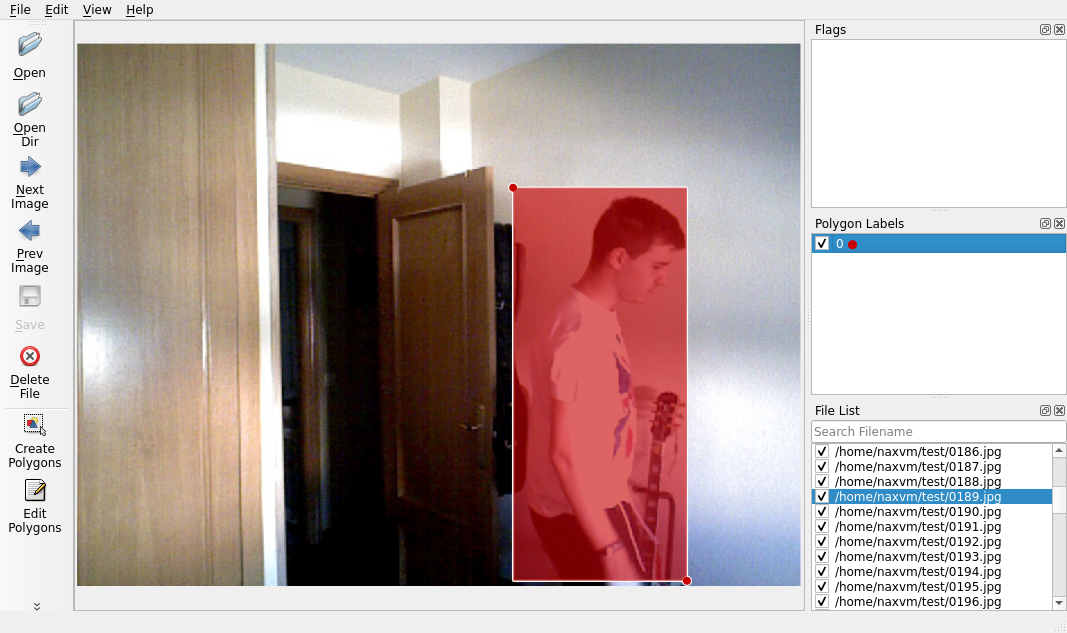
\includegraphics[width=0.8\linewidth]{labelme}
	\caption{Interface of the LabelMe annotation tool \cite{labelme}.}
	\label{fig:3_labelme}
\end{figure}


\section{Person detection experiments}
\label{sec:3_test1}
This experiment compares the two detection architectures implemented on this system: YOLO \cite{yolov3} and SSD\cite{ssd}.

In the case of YOLO, the implemented architecture is YOLOv3, in its \textit{tiny} version. This is due to the memory constraints of the Jetson board where the models are loaded. The available memory (8 GB) has to be shared among TensorFlow and the rest of processes, causing the more memory-intensive models to fail on loading. The YOLOv3 demands too much memory, making impossible to use it properly. Thus, the chosen architecture is a lighter one, publicly available on the YOLO website\footnote{\url{https://pjreddie.com/darknet/yolo/}}: the Tiny YOLOv3 model.

On the other hand, as it was explained in \autoref{sec:1_sota}, on a real-time application the most convenient variant of the SSD-based detectors is the one that uses a MobileNet \cite{mobilenet} as a feature extraction network. The TensorFlow Model Zoo \cite{model_zoo} offers several pre-trained models implementing this network, along which a selection has been carried out (as it will be depicted in other tests). The chosen model integrates a MobileNetv1 whose weights have been quantized \cite{ssd_quantization} in order to reduce the computational cost without reducing the accuracy.\\


In order to quantify the different accuracy vs. inference time tradeoffs that these architectures offer, a specific test has been designed. A specific video sequence has been recorded containing a person wandering across the field of view of the camera. Several extracted frames from this sequence can be observed on \autoref{fig:3_test1_frames}. For every frame on the sequence, the persons are detected using YOLO and SSD respectively, and the IoU and the inference time have been measured, as it can be seen on \autoref{fig:3_test1_results}. Some gaps can be noticed on the detections, corresponding to the frames where the person was out of the sight of the camera.

\begin{figure}[h]
	\centering
	\begin{subfigure}[b]{0.3\linewidth}
		\centering
		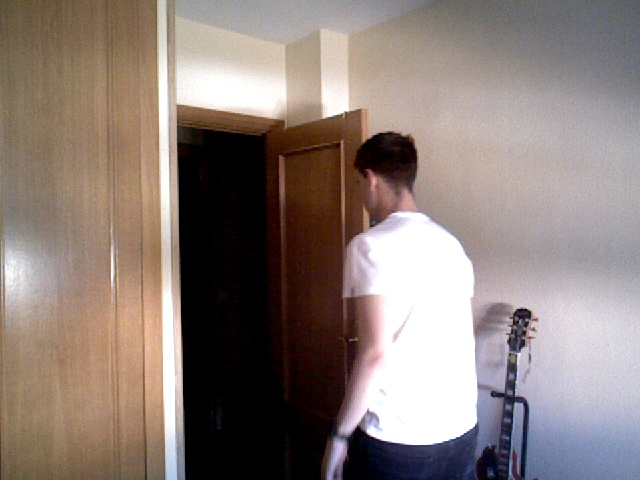
\includegraphics[width=0.95\linewidth]{test1_1}
		\caption{Frame 322.}
	\end{subfigure}
	\begin{subfigure}[b]{0.3\linewidth}
		\centering
		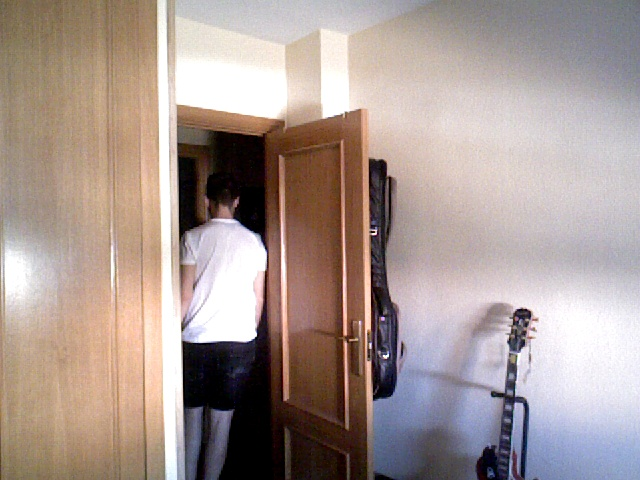
\includegraphics[width=0.95\linewidth]{test1_2}
		\caption{Frame 479.}
	\end{subfigure}
	\begin{subfigure}[b]{0.3\linewidth}
		\centering
		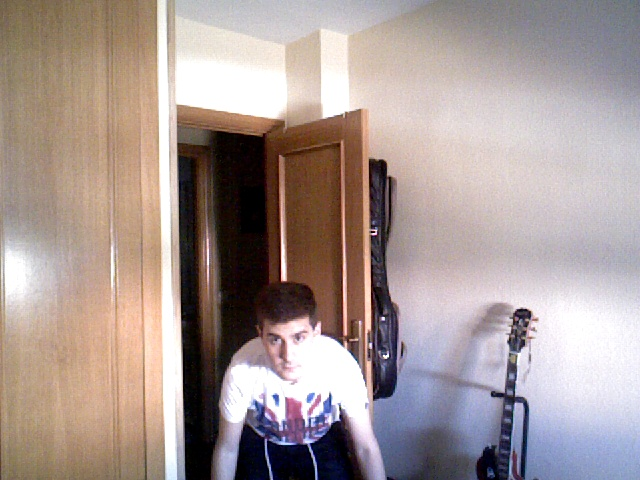
\includegraphics[width=0.95\linewidth]{test1_3}
		\caption{Frame 648.}
	\end{subfigure}
	\caption{3 frames from the test video sequence.}
	\label{fig:3_test1_frames}
\end{figure}




\begin{figure}[h]
	\centering
	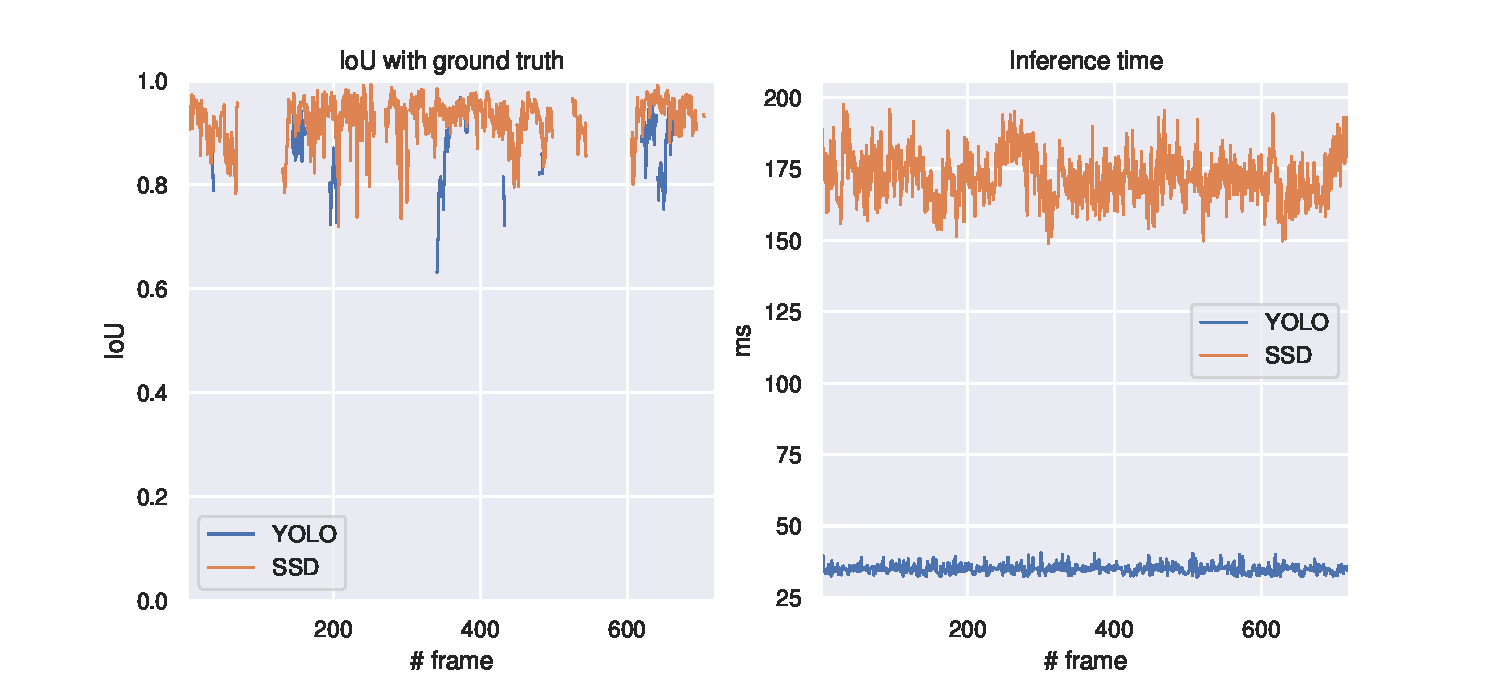
\includegraphics[width=\linewidth]{test1}
	\caption{Results of the person detection test: IoU score with ground truth(left) and inference time per frame (right).}
	\label{fig:3_test1_results}
\end{figure}

\section{Face detection experiments}
\label{sec:3_test2}

One of the improvements of the proposed system over the previous work \cite{tfg} is the utilization of a fully neural detection pipeline, as it was depicted on \autoref{chap:2_materials_methods}. This requires the replacement of the face detection Haar cascade classifier explained on \autoref{sec:1_sota} by a neural alternative: \textit{faced}. This experiment is devoted to compare the performance of both face detection systems.\\

Its design is similar to the previous experiment, using the same video sequence (\autoref{fig:3_test1_frames}) with the ground truth faces labeled using LabelMe. For each frame in the sequence, the faces are extracted using each one of the described methods, and the IoU score is computed with the ground truth face bounding box. The result can be visualized in \autoref{fig:3_test2_results}.

\begin{figure}[h]
	\centering
	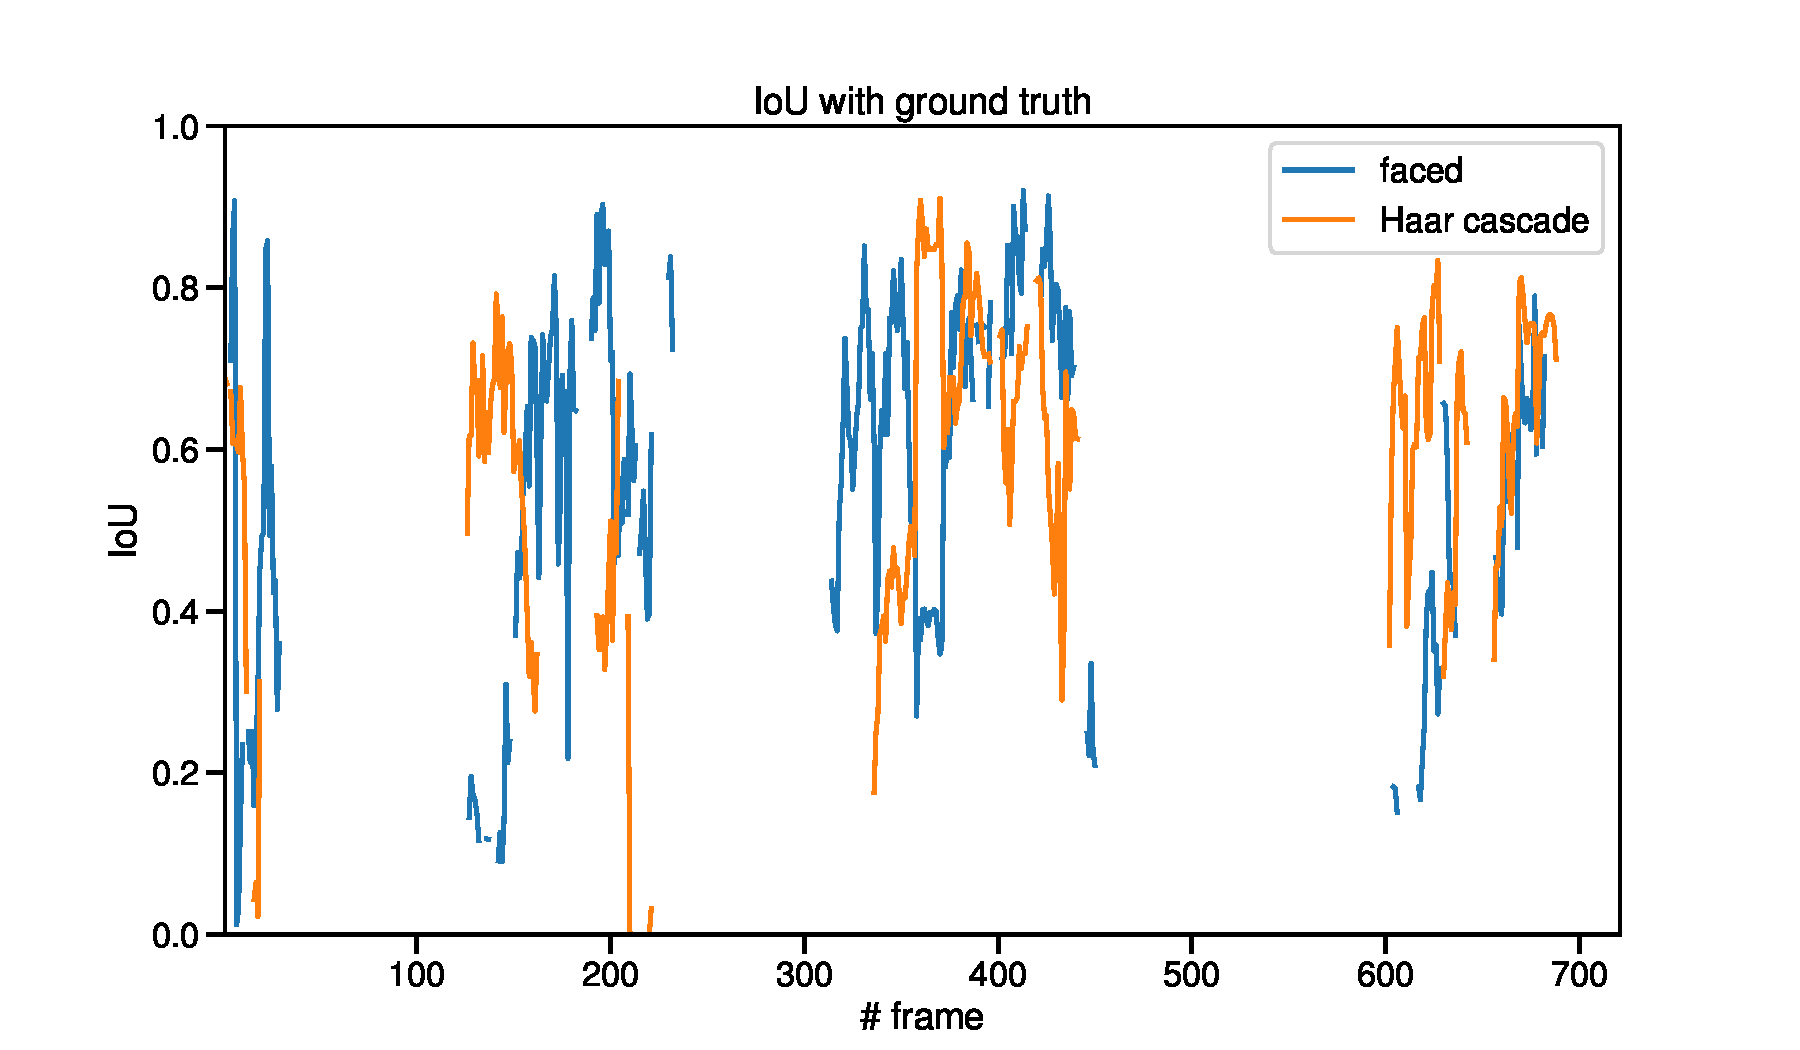
\includegraphics[width=0.6\linewidth]{test2}
	\caption{IoU score with the ground truth for each one of the face detection systems.}
	\label{fig:3_test2_results}
\end{figure}

\section{Face recognition experiments}

\label{sec:3_test4}
The last component of the neural pipeline is a \textit{face recognition} neural network, devoted to confirm the identity of the reference person. This is useful for discerning whether that person has to be followed even if they turns back later, as their position is tracked with the described means. This subsystem is based on a FaceNet \cite{facenet} network, which projects a face into a 128-dimensional space. These projections are used by the proposed system, as their distance to the projection of a reference face is used to determine if the input face belongs to the reference person.\\

This experiment is designed to assess the quality of the projection system, which should yield far points for a different face and near points for a matching face. For this proposal, a video sequence was recorded containing two persons wandering in front of the robot. The faces of each frame are labeled, separating the faces of the two persons in two different classes. A caption of the video with the labels can be seen on \autoref{fig:3_test4_labelme}. \autoref{fig:3_test4_frames} shows several frames from the sequence as well, where some occlusions on the faces can be observed. 

\begin{figure}[h]
	\centering
	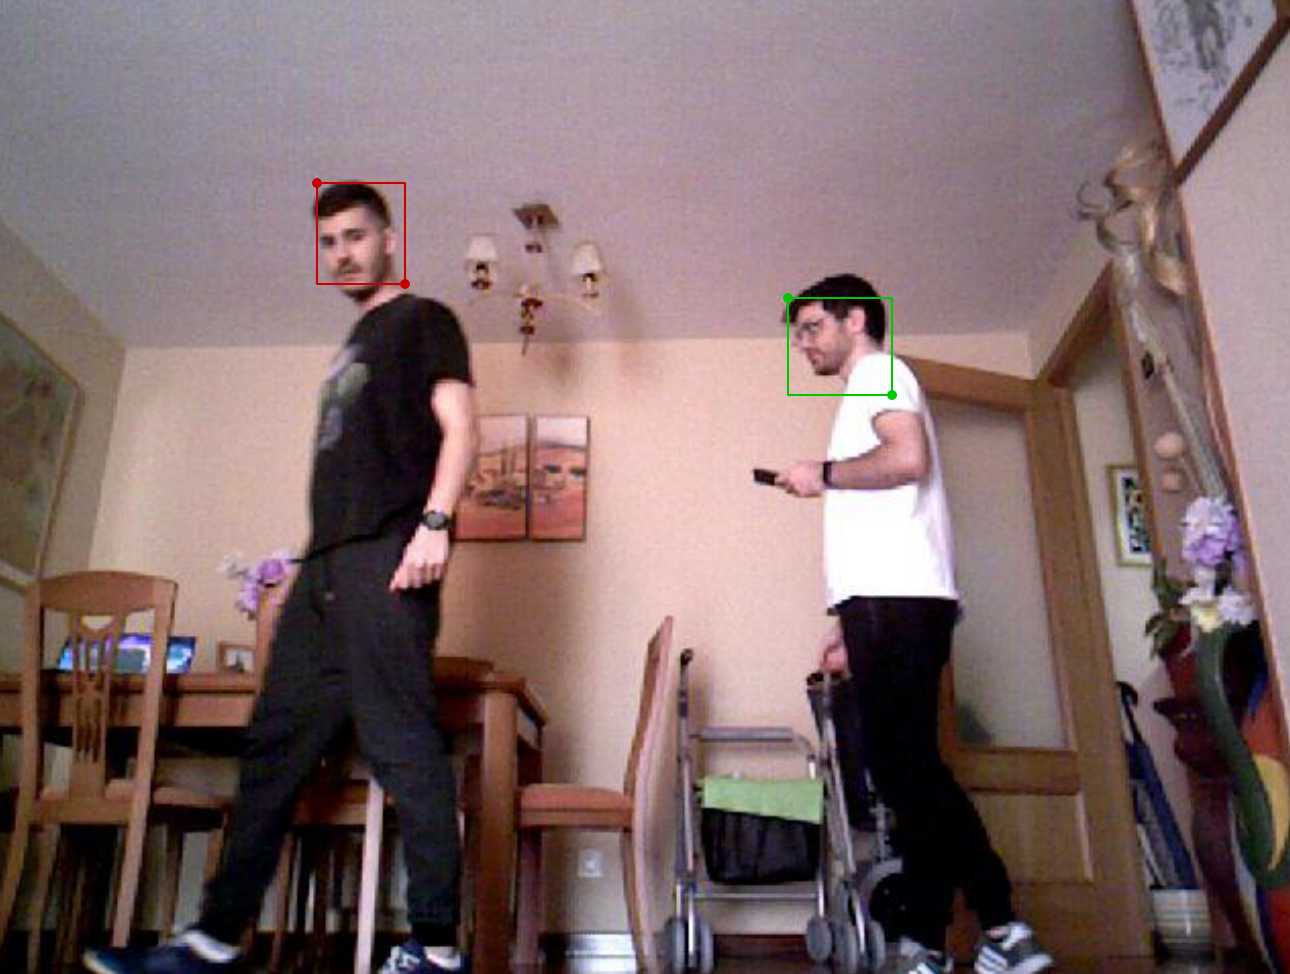
\includegraphics[width=0.6\linewidth]{test4_labelme}
	\caption{A frame of the test sequence showing the labels on the faces.}
	\label{fig:3_test4_labelme}
\end{figure}



\begin{figure}[h]
	\centering
	\begin{subfigure}[b]{0.3\linewidth}
		\centering
		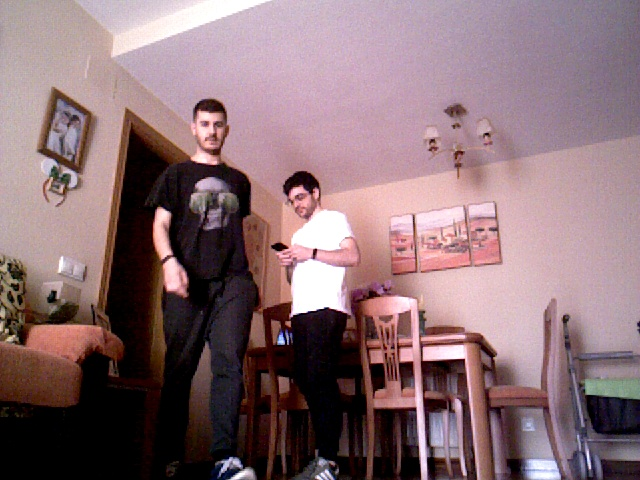
\includegraphics[width=0.95\linewidth]{test4_1}
		\caption{Frame 74.}
	\end{subfigure}
	\begin{subfigure}[b]{0.3\linewidth}
		\centering
		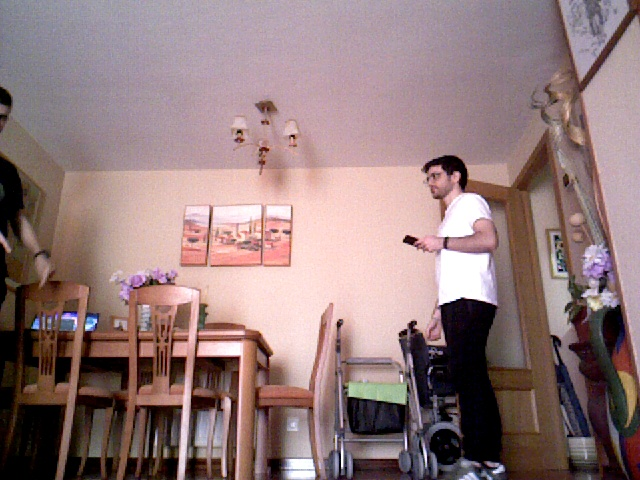
\includegraphics[width=0.95\linewidth]{test4_2}
		\caption{Frame 735.}
	\end{subfigure}
	\begin{subfigure}[b]{0.3\linewidth}
		\centering
		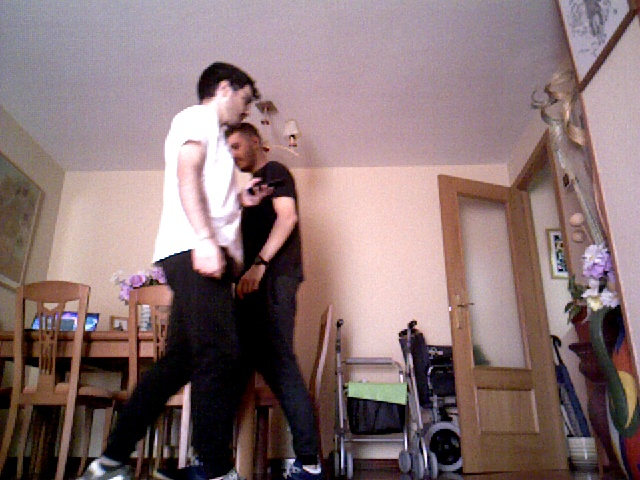
\includegraphics[width=0.95\linewidth]{test4_3}
		\caption{Frame 1136.}
	\end{subfigure}
	\caption{3 frames from the test video sequence.}
	\label{fig:3_test4_frames}
\end{figure}


For computing the distance, the reference face was set using the image on \autoref{fig:3_test4_refface}, and the distance to the reference face of each one of the faces in the video was stored. The result can be observed on \autoref{fig:3_test4_result}.


\begin{figure}[h]
	\centering
	\begin{subfigure}[b]{0.25\linewidth}
		\centering
		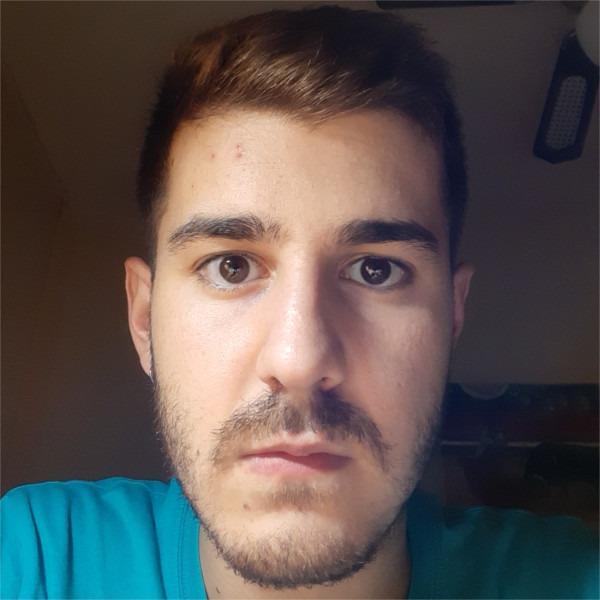
\includegraphics[width=0.95\linewidth]{test4_refface}
		\caption{Image of the reference face.}
		\label{fig:3_test4_refface}
	\end{subfigure}
	\begin{subfigure}[b]{0.7\linewidth}
		\centering
		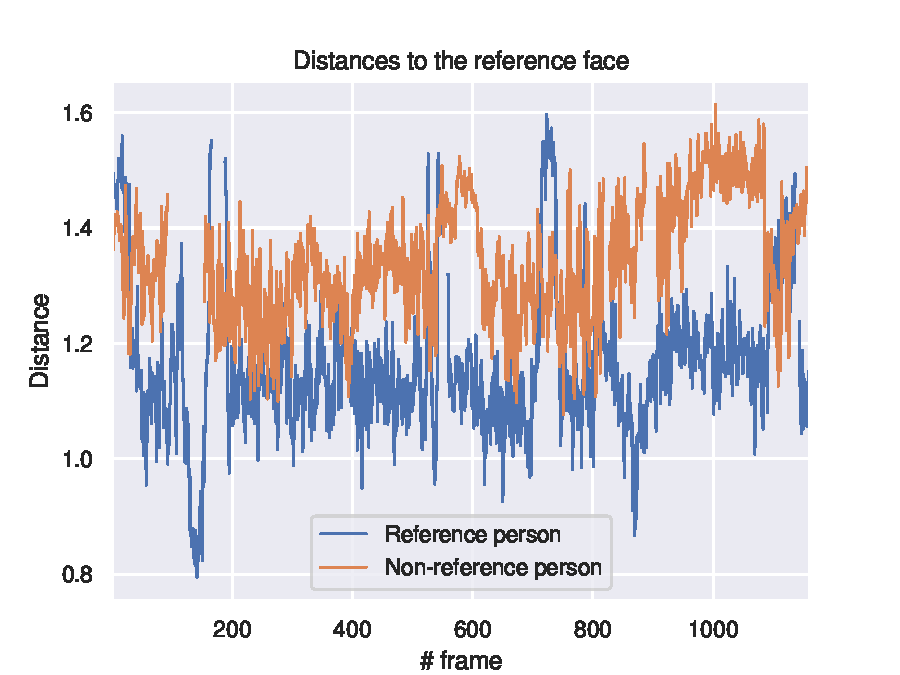
\includegraphics[width=0.95\linewidth]{test4}
		\caption{Resulting distance for the two faces present in the video.}
		\label{fig:3_test4_result}
	\end{subfigure}
	\caption{Results of the face recognition experiments}
	\label{fig:3_test4}
\end{figure}

\section{TensorRT experiments}

\subsection{Performance tuning the optimization parameters}

\label{sec:3_grid_trt}
On \autoref{sec:2_functional_architecture}, the TensorRT engine was introduced. This engine is used to optimize, using a binding component between TensorFlow network graphs and TensorRT itself, the deployment of a neural network on a compatible NVIDIA GPU. There are several tunable parameters for customizing the implementation, and the most relevant ones are described in \autoref{sec:2_functional_architecture} as well. As varying these parameters changes the model size and the inference time, a benchmark has been developed in order to test the inference time of each model. The optimization script performs a grid search between a set of values for each parameter (MSS, MCE and precision mode, as described on \autoref{sec:2_functional_architecture}), and tests the performance on a specific ROSBag sequence, storing the detections and the inference times on a YAML file, besides the optimized graph to be loaded without requiring to perform the optimization again.\\

The inference times for the fastest SSD-based model and the Tiny YOLOv3 implementations are shown below in \autoref{tab:3_ssd_trt_results} and \autoref{tab:3_yolo_trt_results}. The performance tables for the rest of models `can be found in \autoref{chap:annexes}.


\begin{table}[]
	\begin{tabular}{cccc}
		\hline
		\multicolumn{1}{|c|}{\textbf{Precision}}    & \multicolumn{1}{c|}{\textbf{MSS}}        & \multicolumn{1}{c|}{\textbf{MCE}} & \multicolumn{1}{c|}{\textbf{Avg. inference time (ms)}} \\ \hline
		\multicolumn{1}{|c|}{\multirow{9}{*}{FP32}} & \multicolumn{1}{c|}{\multirow{3}{*}{3}}  & \multicolumn{1}{c|}{1}  & \multicolumn{1}{c|}{59,223}    \\ \cline{3-4} 
		\multicolumn{1}{|c|}{}   & \multicolumn{1}{c|}{}          & \multicolumn{1}{c|}{3}  & \multicolumn{1}{c|}{57,139}    \\ \cline{3-4} 
		\multicolumn{1}{|c|}{}   & \multicolumn{1}{c|}{}          & \multicolumn{1}{c|}{5}  & \multicolumn{1}{c|}{58,210}    \\ \cline{2-4} 
		\multicolumn{1}{|c|}{}   & \multicolumn{1}{c|}{\multirow{3}{*}{20}} & \multicolumn{1}{c|}{1}  & \multicolumn{1}{c|}{58,398}    \\ \cline{3-4} 
		\multicolumn{1}{|c|}{}   & \multicolumn{1}{c|}{}          & \multicolumn{1}{c|}{3}  & \multicolumn{1}{c|}{58,240}    \\ \cline{3-4} 
		\multicolumn{1}{|c|}{}   & \multicolumn{1}{c|}{}          & \multicolumn{1}{c|}{5}  & \multicolumn{1}{c|}{57,910}    \\ \cline{2-4} 
		\multicolumn{1}{|c|}{}   & \multicolumn{1}{c|}{\multirow{3}{*}{50}} & \multicolumn{1}{c|}{1}  & \multicolumn{1}{c|}{41,077}    \\ \cline{3-4} 
		\multicolumn{1}{|c|}{}   & \multicolumn{1}{c|}{}          & \multicolumn{1}{c|}{3}  & \multicolumn{1}{c|}{41,410}    \\ \cline{3-4} 
		\multicolumn{1}{|c|}{}   & \multicolumn{1}{c|}{}          & \multicolumn{1}{c|}{5}  & \multicolumn{1}{c|}{41,080}    \\ \hline
		\multicolumn{1}{|c|}{\multirow{9}{*}{FP16}} & \multicolumn{1}{c|}{\multirow{3}{*}{3}}  & \multicolumn{1}{c|}{1}  & \multicolumn{1}{c|}{57,423}    \\ \cline{3-4} 
		\multicolumn{1}{|c|}{}   & \multicolumn{1}{c|}{}          & \multicolumn{1}{c|}{3}  & \multicolumn{1}{c|}{56,777}    \\ \cline{3-4} 
		\multicolumn{1}{|c|}{}   & \multicolumn{1}{c|}{}          & \multicolumn{1}{c|}{5}  & \multicolumn{1}{c|}{57,286}    \\ \cline{2-4} 
		\multicolumn{1}{|c|}{}   & \multicolumn{1}{c|}{\multirow{3}{*}{20}} & \multicolumn{1}{c|}{1}  & \multicolumn{1}{c|}{56,783}    \\ \cline{3-4} 
		\multicolumn{1}{|c|}{}   & \multicolumn{1}{c|}{}          & \multicolumn{1}{c|}{3}  & \multicolumn{1}{c|}{56,591}    \\ \cline{3-4} 
		\multicolumn{1}{|c|}{}   & \multicolumn{1}{c|}{}          & \multicolumn{1}{c|}{5}  & \multicolumn{1}{c|}{56,637}    \\ \cline{2-4} 
		\multicolumn{1}{|c|}{}   & \multicolumn{1}{c|}{\multirow{3}{*}{50}} & \multicolumn{1}{c|}{1}  & \multicolumn{1}{c|}{40,053}    \\ \cline{3-4} 
		\multicolumn{1}{|c|}{}   & \multicolumn{1}{c|}{}          & \multicolumn{1}{c|}{3}  & \multicolumn{1}{c|}{\textbf{39,738}}    \\ \cline{3-4} 
		\multicolumn{1}{|c|}{}   & \multicolumn{1}{c|}{}          & \multicolumn{1}{c|}{5}  & \multicolumn{1}{c|}{40,115}    \\ \hline
		\multicolumn{1}{|c|}{\multirow{9}{*}{INT8}} & \multicolumn{1}{c|}{\multirow{3}{*}{3}}  & \multicolumn{1}{c|}{1}  & \multicolumn{1}{c|}{62,859}    \\ \cline{3-4} 
		\multicolumn{1}{|c|}{}   & \multicolumn{1}{c|}{}          & \multicolumn{1}{c|}{3}  & \multicolumn{1}{c|}{61,105}    \\ \cline{3-4} 
		\multicolumn{1}{|c|}{}   & \multicolumn{1}{c|}{}          & \multicolumn{1}{c|}{5}  & \multicolumn{1}{c|}{62,383}    \\ \cline{2-4} 
		\multicolumn{1}{|c|}{}   & \multicolumn{1}{c|}{\multirow{3}{*}{20}} & \multicolumn{1}{c|}{1}  & \multicolumn{1}{c|}{62,439}    \\ \cline{3-4} 
		\multicolumn{1}{|c|}{}   & \multicolumn{1}{c|}{}          & \multicolumn{1}{c|}{3}  & \multicolumn{1}{c|}{61,810}    \\ \cline{3-4} 
		\multicolumn{1}{|c|}{}   & \multicolumn{1}{c|}{}          & \multicolumn{1}{c|}{5}  & \multicolumn{1}{c|}{63,477}    \\ \cline{2-4} 
		\multicolumn{1}{|c|}{}   & \multicolumn{1}{c|}{\multirow{3}{*}{50}} & \multicolumn{1}{c|}{1}  & \multicolumn{1}{c|}{46,123}    \\ \cline{3-4} 
		\multicolumn{1}{|c|}{}   & \multicolumn{1}{c|}{}          & \multicolumn{1}{c|}{3}  & \multicolumn{1}{c|}{46,835}    \\ \cline{3-4} 
		\multicolumn{1}{|c|}{}   & \multicolumn{1}{c|}{}          & \multicolumn{1}{c|}{5}  & \multicolumn{1}{c|}{47,387}    \\ \hline
		\multicolumn{3}{|c|}{GPU without TensorRT}       & \multicolumn{1}{c|}{172,269}   \\ \hline
		\multicolumn{3}{|c|}{CPU}        & \multicolumn{1}{c|}{112,111}   \\ \hline
	\end{tabular}
	\caption{Grid search results for the \texttt{ssd\_mobilenet\_v1\_0.75\_depth\_coco} model. The lowest inference time is \textbf{boldfaced}.}
	\label{tab:3_ssd_trt_results}
\end{table}


\begin{table}[]
	\begin{tabular}{|c|c|c|c|}
		\hline
		\textbf{Precision}    & \textbf{MSS}        & \textbf{MCE} & \textbf{Avg. inference time (ms)} \\ \hline
		\multirow{9}{*}{FP32} & \multirow{3}{*}{3}  & 1  & 20,898    \\ \cline{3-4} 
		&  & 3  & 21,032    \\ \cline{3-4} 
		&  & 5  & 21,112    \\ \cline{2-4} 
		& \multirow{3}{*}{20} & 1  & 21,373    \\ \cline{3-4} 
		&  & 3  & 21,208    \\ \cline{3-4} 
		&  & 5  & 21,639    \\ \cline{2-4} 
		& \multirow{3}{*}{50} & 1  & 22,506    \\ \cline{3-4} 
		&  & 3  & 22,301    \\ \cline{3-4} 
		&  & 5  & 22,239    \\ \hline
		\multirow{9}{*}{FP16} & \multirow{3}{*}{3}  & 1  & 16,180    \\ \cline{3-4} 
		&  & 3  & \textbf{15,922  }  \\ \cline{3-4} 
		&  & 5  & 16,061    \\ \cline{2-4} 
		& \multirow{3}{*}{20} & 1  & 16,200    \\ \cline{3-4} 
		&  & 3  & 16,208    \\ \cline{3-4} 
		&  & 5  & 16,183    \\ \cline{2-4} 
		& \multirow{3}{*}{50} & 1  & 18,294    \\ \cline{3-4} 
		&  & 3  & 18,110    \\ \cline{3-4} 
		&  & 5  & 18,248    \\ \hline
		\multirow{9}{*}{INT8} & \multirow{3}{*}{3}  & 1  & 35,266    \\ \cline{3-4} 
		&  & 3  & 36,329    \\ \cline{3-4} 
		&  & 5  & 36,289    \\ \cline{2-4} 
		& \multirow{3}{*}{20} & 1  & 36,305    \\ \cline{3-4} 
		&  & 3  & 35,420    \\ \cline{3-4} 
		&  & 5  & 35,734    \\ \cline{2-4} 
		& \multirow{3}{*}{50} & 1  & 35,195    \\ \cline{3-4} 
		&  & 3  & 34,815    \\ \cline{3-4} 
		&  & 5  & 35,178    \\ \hline
		\multicolumn{3}{|c|}{GPU without TensorRT}       & 35,996    \\ \hline
		\multicolumn{3}{|c|}{CPU}          & NHWC      \\ \hline
	\end{tabular}
	\caption{Grid search results for the \texttt{yolo\_v3\_tiny} model. The lowest inference time is \textbf{boldfaced}. The CPU inferences could not be performed due to hardware incompatibility issues.}
	\label{tab:3_yolo_trt_results}
\end{table}

\subsection{Optimized graphs vs. standard graphs}

\label{sec:3_test3}
As it has been studied, tuning the TensorRT optimization parameters greatly varies the inference time required for processing an image. However, as it was explained in \autoref{sec:2_functional_architecture}, this acceleration additionally entails a reduction on the precision, as the weights of the neural network layers are trimmed in the process. The precision mode choice determines the precision of the weights. In the case of the SSD-MobileNet detector, the best inference time (\autoref{tab:3_ssd_trt_results}) was yielded by the FP16 precision mode, which trims the weights to a 16-bit long floating point number. This will cause the inference precision to be reduced as the operations are performed on a coarser mode.\\

This experiment aims to quantify the loss of precision when the SSD model is optimized by TensorRT using the FP16 precision model, which is the fastest mode to infer, as shown in \autoref{tab:3_ssd_trt_results}. To do so, the test sequence (\autoref{fig:3_test1_frames}) is used again, passing each frame forward on the standard neural network and storing the detected persons. Later, the same video sequence is passed through the TensorRT version of the same graph, storing the detections of each person as well. When both passes are performed, the IoU score is computed on each frame between the standard inferences (considered the ground-truth labels) and the TensorRT inferences. This IoU score on each frame, along with the inference times for each network model, can be seen on \autoref{fig:3_std_vs_trt}.

\begin{figure}[h]
	\centering
	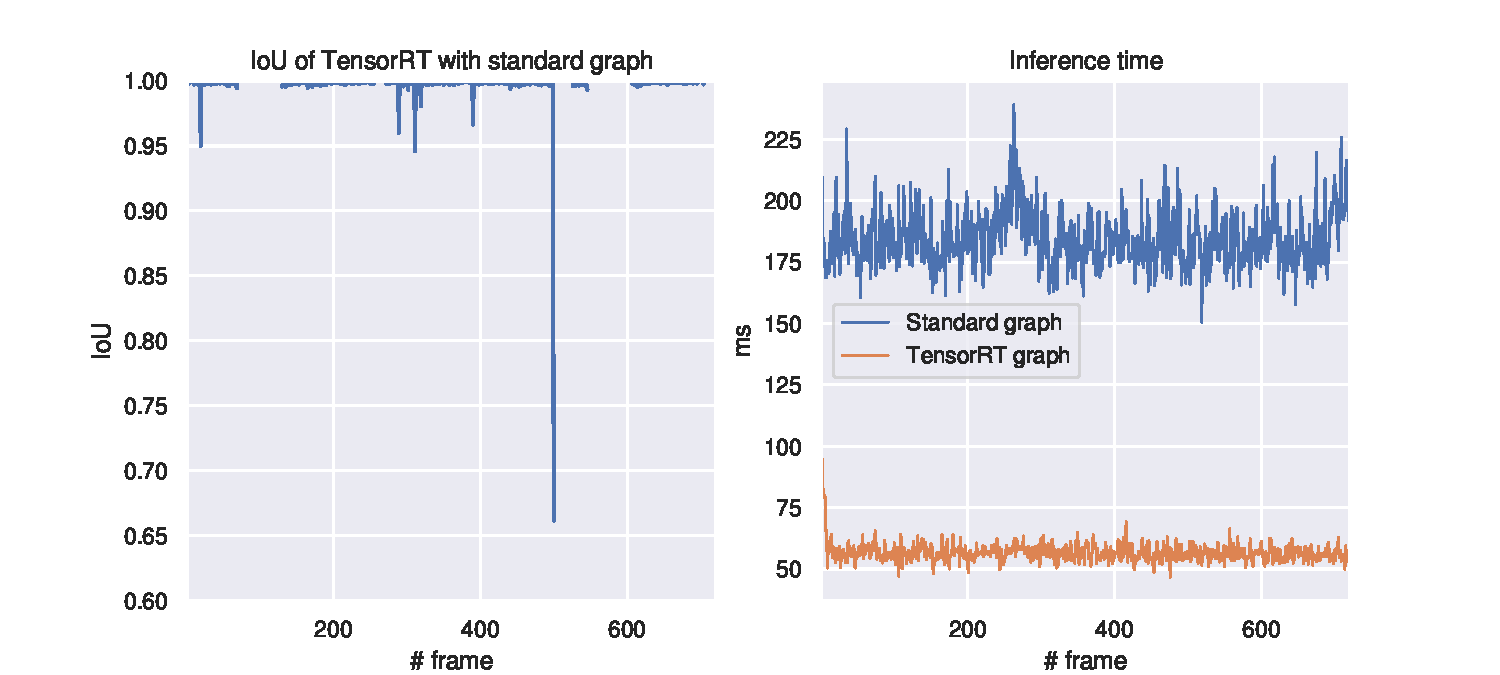
\includegraphics[width=0.85\linewidth]{test3}
	\caption{IoU between the standard graph and the TensorRT graph inferences (left) and inference times for both networks (right). The IoU graph has been rescaled between 0.6 and 1 to have a better visualization of the IoU variability.}
	\label{fig:3_std_vs_trt}
\end{figure}






\section{Motion tracker experiments}

\label{sec:3_test5}
In \autoref{sec:2_functional_architecture}, the Lucas-Kanade tracker was described. This tracker aims to follow the movements of the person between two consecutive inferences from the neural pipeline. As in embedded systems these inferences might take a long time, an interpolation of the detections using optical flow can be crucial for avoiding a loss of the location of the person, especially if a partial occlusion of the person causes that the network does not detect them for a while.\\

This experiment aims to identify the conditions under which a tracker can palliate these drawbacks of the neural detection pipeline, depending on the parameter $k$. This $k$ modulates the number of elapsed frames between two consecutive neural detections, and takes a higher value if the inferences take longer to be computed by the neural pipeline. On the test, a specific test sequence was recorded and labeled, using a hanging blanket with the purpose of partially occlude the person, making the network to lose the detections. Several frames of the sequence can be visualized on \autoref{fig:3_test5_frames}.\\


\begin{figure}[h]
	\centering
	\begin{subfigure}[b]{0.3\linewidth}
		\centering
		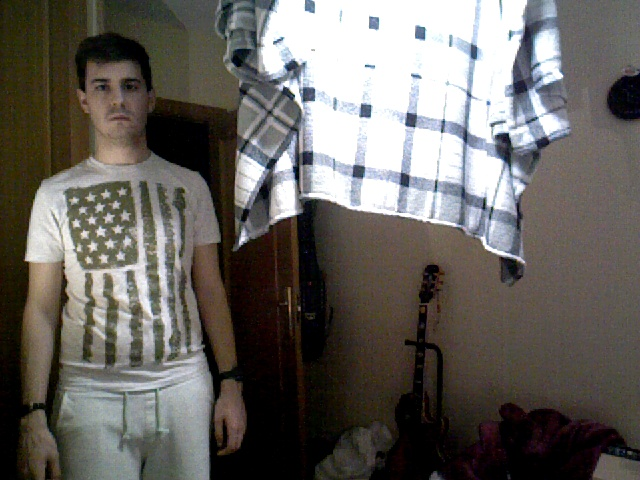
\includegraphics[width=0.95\linewidth]{test5_1}
		\caption{Frame 285.}
	\end{subfigure}
	\begin{subfigure}[b]{0.3\linewidth}
		\centering
		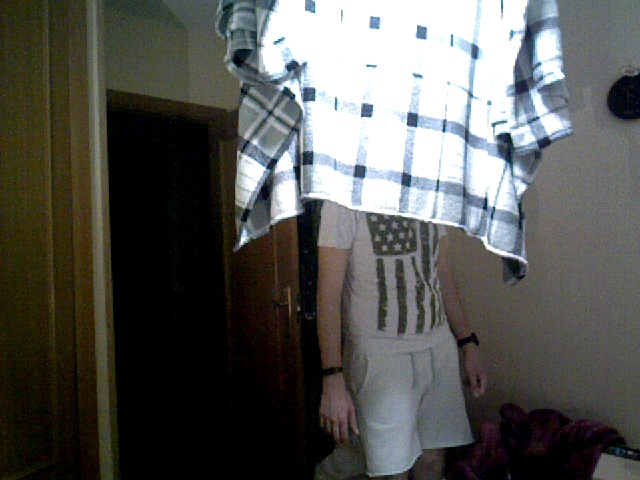
\includegraphics[width=0.95\linewidth]{test5_2}
		\caption{Frame 788.}
	\end{subfigure}
	\begin{subfigure}[b]{0.3\linewidth}
		\centering
		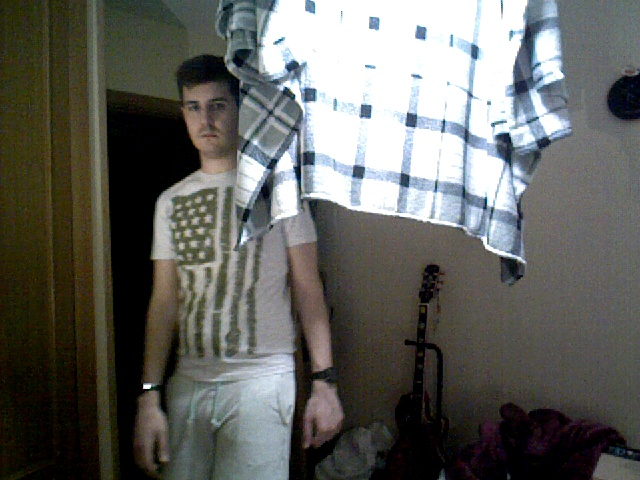
\includegraphics[width=0.95\linewidth]{test5_3}
		\caption{Frame 864.}
	\end{subfigure}
	\caption{3 frames from the test video sequence.}
	\label{fig:3_test5_frames}
\end{figure}



A correctly tuned tracker maintains the detection and moves the bounding box for a number of frames (determined by the \textit{patience} parameter, as described in \autoref{sec:2_functional_architecture}). The video sequence was evaluated using $k=10$ and $k=20$, checking the influence of the tracker in the IoU with the ground truth labels of the sequence. The result for both values of $k$ can be observed on \autoref{fig:3_test5}, where the lapse corresponding to the person occlusion has been emphasized.

\begin{figure}[h]
	\centering
	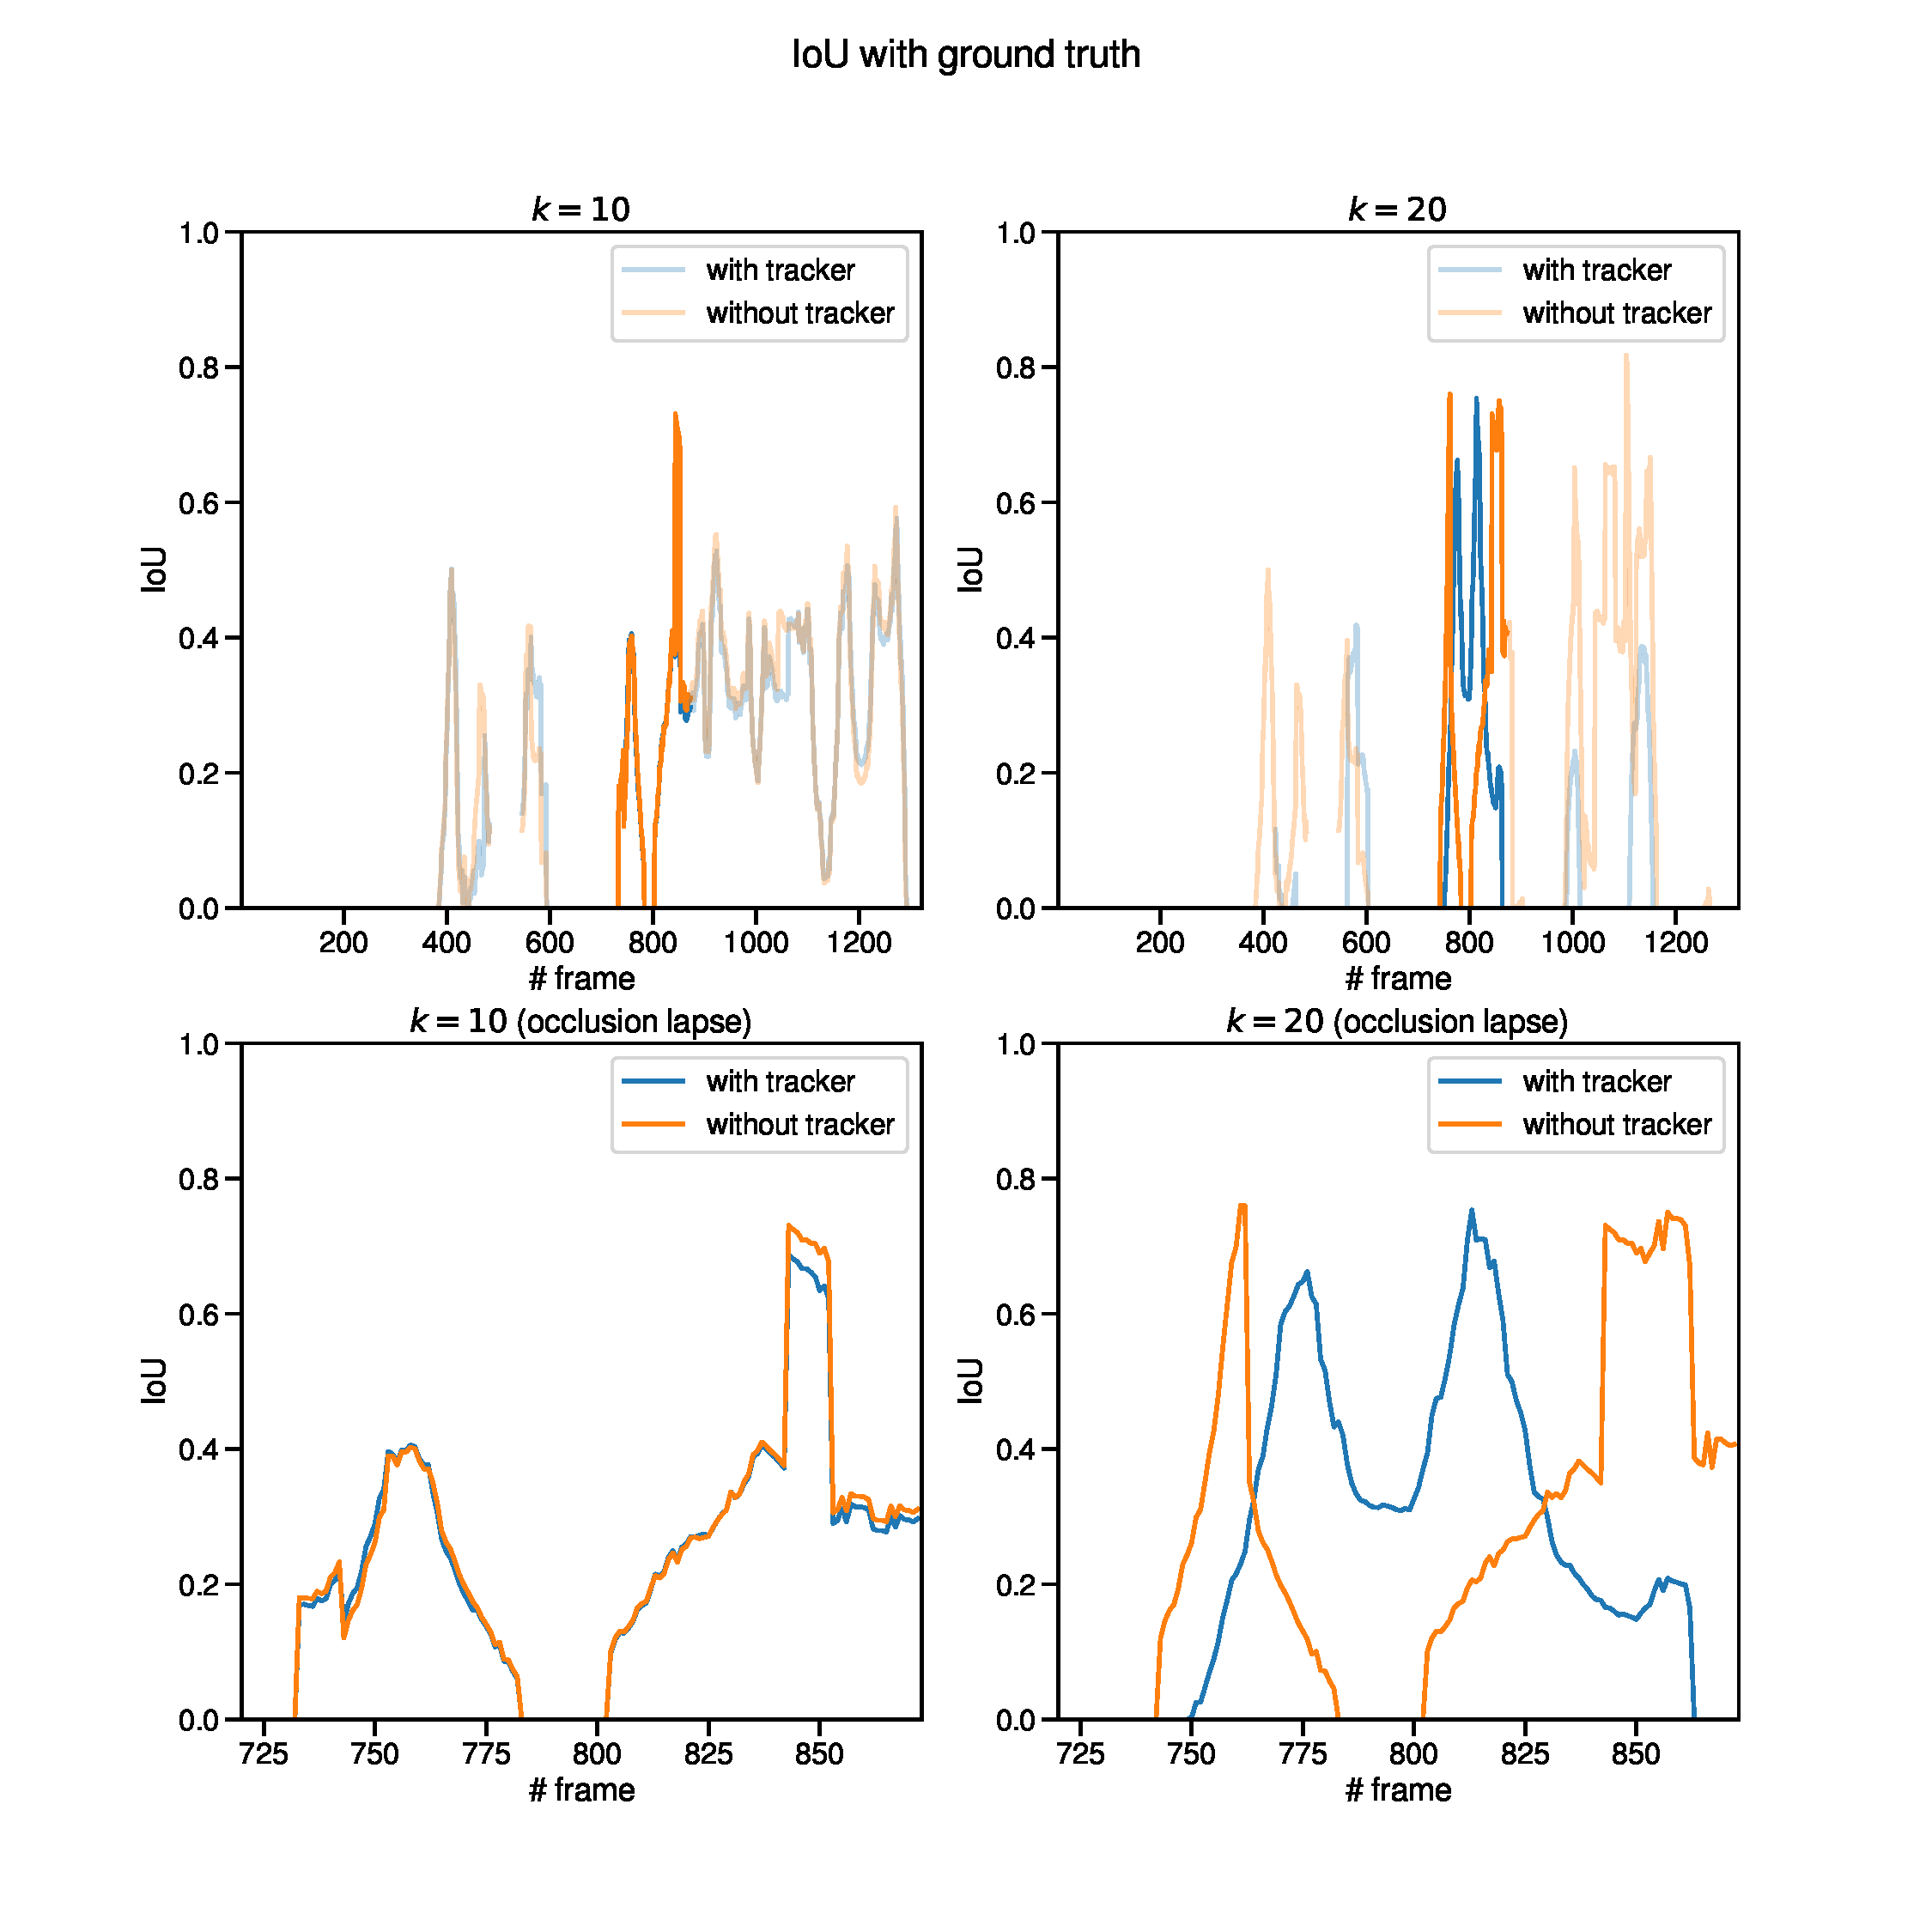
\includegraphics[width=0.85\linewidth]{test5}
	\caption{Results of the motion tracker test. The lapse corresponding to the person occlusion has been emphasized.}
	\label{fig:3_test5}
\end{figure}



\section{Global system experiments}

Finally, a visual assessment can be derived from a sample of the fully functional system\footnote{\url{https://www.youtube.com/watch?v=WZ0riKMwJWA}}. As it can be seen on \autoref{fig:3_testfull_frames}, the behavior followed by the robot is the expected one.

\begin{figure}[h]
	\centering
	\begin{subfigure}[t]{0.3\linewidth}
		\centering
		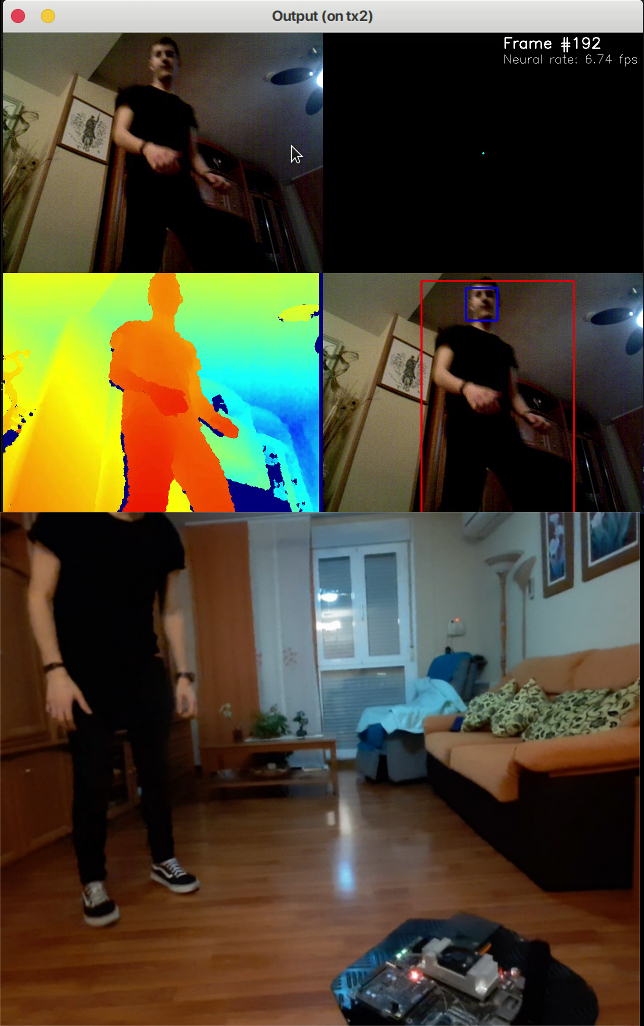
\includegraphics[width=0.95\linewidth]{testfull_1}
		\caption{Person detection.}
	\end{subfigure}
	\begin{subfigure}[t]{0.3\linewidth}
		\centering
		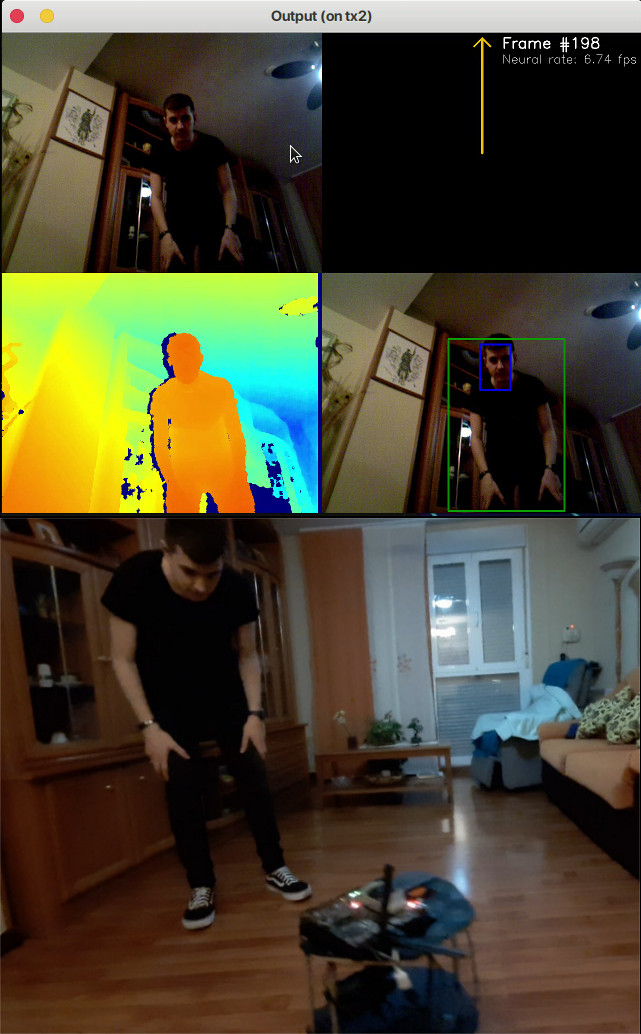
\includegraphics[width=0.95\linewidth]{testfull_2}
		\caption{Person recognition and following.}
	\end{subfigure}
	\begin{subfigure}[t]{0.3\linewidth}
		\centering
		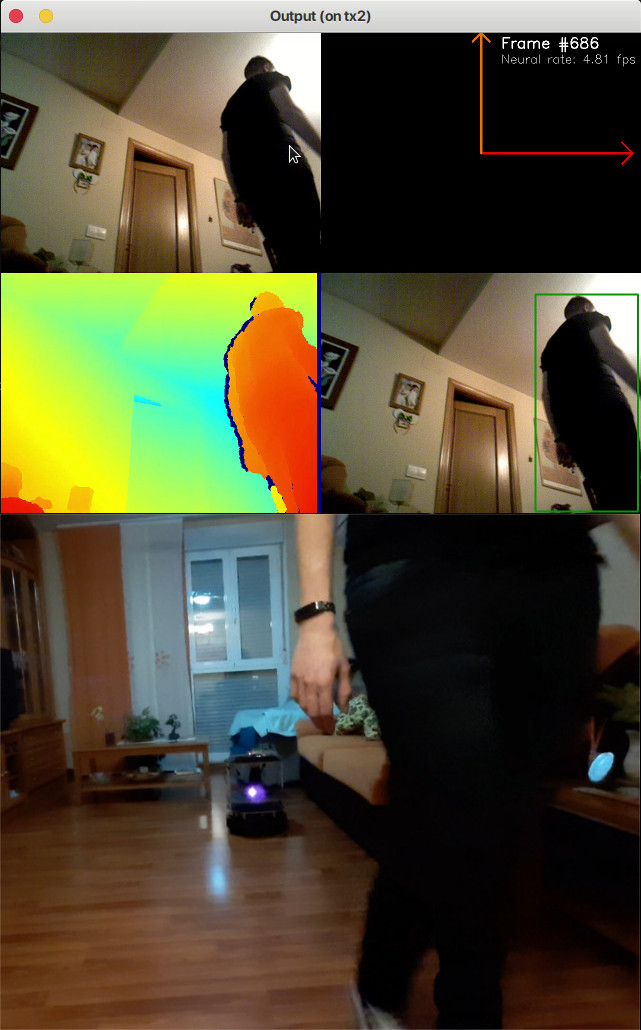
\includegraphics[width=0.95\linewidth]{testfull_3}
		\caption{Following without face feedback.}
	\end{subfigure}
	\caption{3 frames from the full test (available on YouTube).}
	\label{fig:3_testfull_frames}
\end{figure}



